
\noindent 
\textbf{\stepcounter{zadatak}
\thecjelina.\thezadatak.}
Koliki je iznos ubrzanja blokova vezanih nerastezljivom niti prikazanih na slici? Kutovi su 
$\alpha=40 ^\circ$  i $\beta=50^\circ $, a mase blokova $m_A=4\ kg$ i $m_B=6\ kg$ . Trenje se zanemaruje.

\begin{figure}[ht]%{r}{0.7\textwidth} % Inline image example
  \begin{center}
    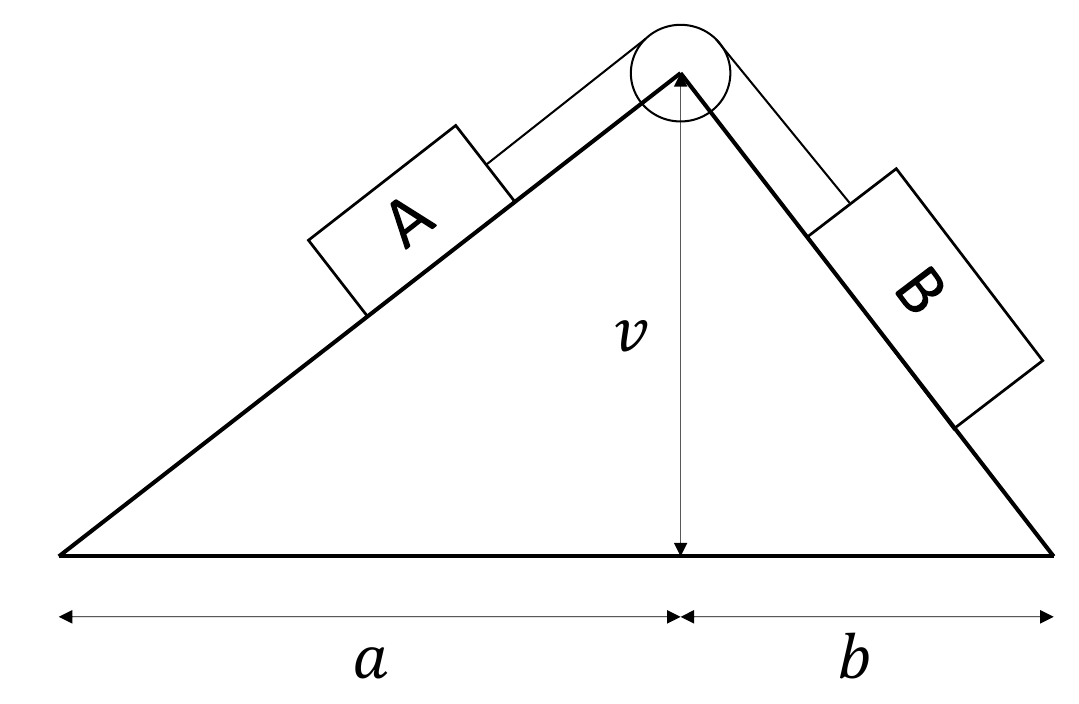
\includegraphics[scale=0.20]{03_Dinamika_materijalne_tocke/kosina_5_3.png}
  \end{center}
  %\caption{Fish}
\end{figure}

%^\circ
